\chapter{Workflow}
Nei Capitoli~\ref{cap:deployment} e \ref{cap:tracing-metrics} abbiamo visto come l'applicazione car rental, descritta nel Capitolo~\ref{cap:app}, viene rilasciata su Minikube e come possiamo analizzare metriche e workflow.

In questo capitolo ci concentriamo invece proprio sul workflow. Prima di qualunque modifica, \textit{Car-Rental} aveva un workflow esclusivamente sequenziale: quando un utente invocava una qualunque operazione tramite \textit{users-service}, la sequenza di chiamate agli altri microservizio era puramente sincrona e determinstica, cioè era sempre la stessa data l'operazione chiamata.

Per capire meglio osserviamo il workflow di una prenotazione da parte di un utente, mostrato in Figura~\ref{fig:jaeger_reservation}. Quando un utente chiama \texttt{reserve} tramite l'interfaccia grafica, si genere sempre la stessa cascata di chiamate; ovviamente i tempi di esecuzione variano di chiamata in chiamata.

\myskip

Il nostro obiettivo è adesso complicare questo workflow; faremo riferimento sempre a quello descritto sopra. Facendo riferimento alla terminogia usata nell'articolo del tool Eulero~\cite{carnevali2023compositional}, che useremo più avanti, l'applicazione prima della modifica combina solamente blocchi di tipo sequenziale (SEQ), mentre a noi interessa aggiungere degli blocchi XOR e blocchi AND, che sono descritti nella Sezione~\ref{sec:blocchi}.

%%%%%%%%%%%%%%%%%%%%%%%%%%%%%%%%%%%%%%%%%%%%%%%%%%
\section{Blocchi (MODIFICARE DOPO L'IMPLEMENTAZIONE)}
\label{sec:blocchi}
Vediamo come prima cosa quali blocchi sono stati aggiunti e in che punto dell'attuale workflow sono stati eseguiti. I nomi di questi microservizi non hanno una qualche logica complicata, ma ci servono solo per tenere traccia di come il flusso sta eseguendo. Considereremo la traccia fornita come esempio nella Figura~\ref{fig:jaeger_reservation}.
\begin{figure}[htbp]
    \centering
    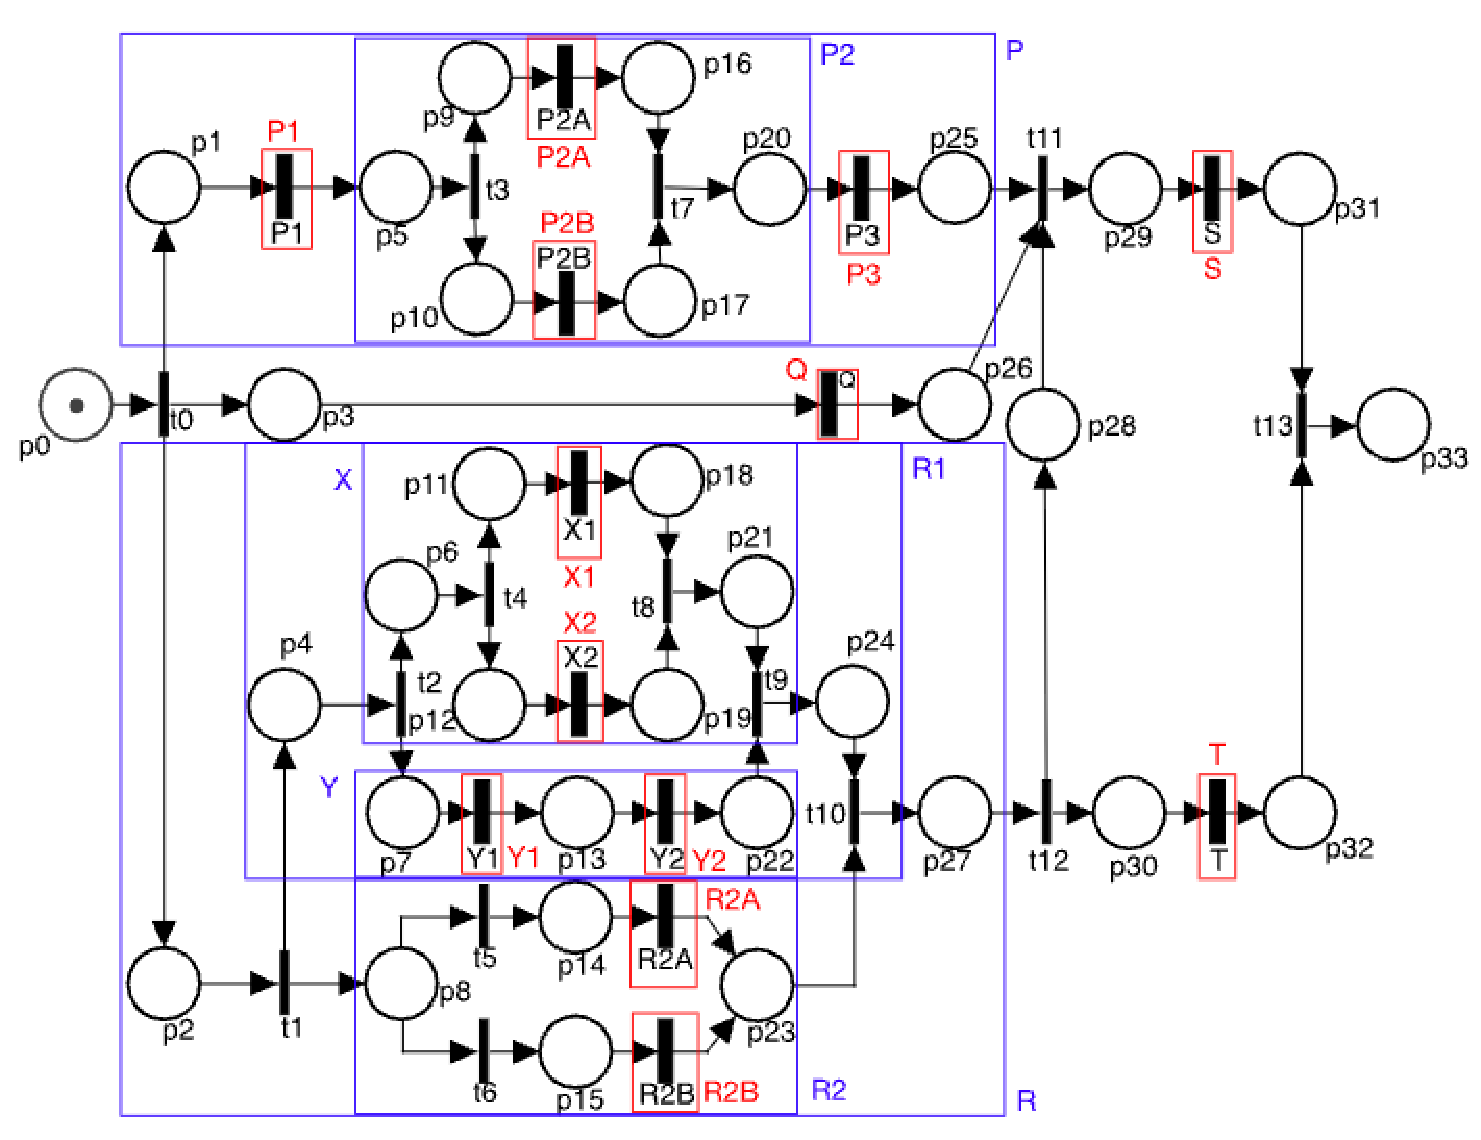
\includegraphics[width=.8\textwidth]{images/5-workflow/STPN.pdf}
    \caption{Stochastic Time Petri Net example~\cite{carnevali2023compositional}.}
    \label{fig:STPN}
\end{figure}

\subsection{XOR}
I blocchi XOR, come mostrato in R2 in Figura~\ref{fig:STPN}, rappresentano scelte casuali esclusive definite da una certa probabilità. Questo vuol dire che se abbiamo $n$ possibili strade che il flusso può prendere, ne sarà scelta una e una soltanto in base alla probabilità assegnata.

Nella nostra applicazione è stato aggiunto un blocco XOR tra i microservizi \textit{users-service} e \textit{reservation-service}. Il blocco è così composto:
\begin{itemize}
    \item Un nodo iniziale chiamato da \textit{users-service} che prende una scelta randomica sul prossimo servizio da chiamare.
    \item Tre possibili servizi che implementano una busy wait per un tempo campionato da una qualche distribuzione.
    \item Un nodo finale che restiuisce il comando a \textit{reservation-service}.
\end{itemize}

\subsection{AND}
I blocchi AND, come mostrato in X in Figura~\ref{fig:STPN}, rappresentano esecuzioni indipendenti che possono essere eseguite in parallelo. Questo vuol dire che se abbiamo $n$ strade, tutte saranno eseguite contemporaneamente e si sincronizzeranno alla fine.
Nella nostra applicazione è stato aggiunto un blocco AND tra i microservizi \textit{billing-service} e \textit{rental-service}. Il blocco è così composto:
\begin{itemize}
    \item Un nodo iniziale chiamato da \textit{billing-service} che chiama in parallelo i tre componenti successivi.
    \item Tre servizi che implementano una busy wait per un tempo campionato da una qualche distribuzione.
    \item Un nodo finale sul quale i tre precedenti componenti si sincronizzano e che successivamente restiuisce il comando a \textit{rental-service}.
\end{itemize}

%%%%%%%%%%%%%%%%%%%%%%%%%%%%%%%%%%%%%%%%%%%%%%%%%%
\section{Implementazione}
Non è importante cosa i nuovi blocchi facciano, cioè non sarà implementato un qualche aspetto funzionale; il loro obiettivo è, come detto, solamente quello di complicare il workflow.

A livello implementativo i blocchi che andremo ad aggiungere non devono essere funzionali, cioè non devono aggiungere una qualche funzionalità applicazione, ma devono solo servire appunto per complicare il workflow.